\documentclass{article}
\usepackage[utf8]{inputenc}

\title{MATH2710 — Portfolio 1.1 - 1.4}
\author{Mike Medved}
\date{January 27th, 2022}

\usepackage{color}
\usepackage{amsthm}
\usepackage{amssymb} 
\usepackage{amsmath}
\usepackage{lmodern}
\usepackage{mathtools, nccmath}
\usepackage{listings}
\usepackage[margin=1in]{geometry} 
\usepackage[dvipsnames]{xcolor}
\usepackage{tikz}

\usepackage{xparse}
%
\DeclarePairedDelimiterX{\set}[1]{\{}{\}}{\setargs{#1}}
\NewDocumentCommand{\setargs}{>{\SplitArgument{1}{;}}m}
{\setargsaux#1}
\NewDocumentCommand{\setargsaux}{mm}
{\IfNoValueTF{#2}{#1} {#1\,\delimsize|\,\mathopen{}#2}}%{#1\:;\:#2}

\parindent = 0pt

\newtheorem*{thm}{Theorem}

\begin{document}

\maketitle

\section{Deliverables}

\subsection{Sets}

\subsubsection{Finite Sets}

A finite set is a set that contains a finite amount of elements. For example, the sets $A = \{1, 2, 3\}$ and $B = \{1, 2, 3, 4, 5\}$ are both finite sets.

\subsubsection{Countably Infinite Sets}

A countably infinite set is a set that contains an infinite amount of elements, but can be put into a one-to-one correspondence with the natural numbers. For example, the set $C = \{1, 2, 3, 4, 5, \ldots\}$ is a countably infinite set. Similarly, the natural numbers $\mathbb{N}$ themselves are a countably infinite set.

\subsubsection{Uncountably Infinite Sets}

A uncountably infinite set is a set that contains an infinite amount of elements, but cannot be put into a one-to-one correspondence with the natural numbers. For example, the set $D = \{1, 2, 3, 4, 5, \ldots, \frac{1}{2}, \frac{1}{3}, \frac{1}{4}, \ldots\}$ is a uncountably infinite set. Similarly, the real numbers $\mathbb{R}$ themselves are a uncountably infinite set.

\subsection{Sets Inclusivity with respect to the Reals}

\begin{figure}[!htb]
    \centering
    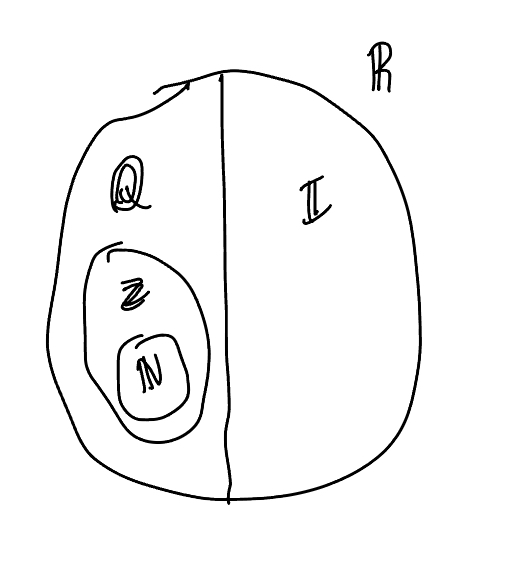
\includegraphics[scale=0.2]{inclusivity.jpeg}
    \caption{Inclusivity of $\mathbb{N}, \mathbb{Z}, \text{ and }\mathbb{Q},$ with respect to $\mathbb{R}$}
\end{figure}

\newpage
\subsection{Intervals}

\subsubsection{$(a, b)$}

An interval $(a, b)$ is a set of all real numbers $x$ such that $a < x < b$. Some examples of intervals on $(a, b)$ are $(0, 1)$ and $(10, 100)$.

\subsubsection{$(a, \infty)$}

An interval $(a, \infty)$ is a set of all real numbers $x$ such that $a < x$. Some examples of intervals on $(a, \infty)$ are $(0, \infty)$ and $(10, \infty)$.

\subsection{Cartesian Products}

\subsubsection{Two Sets}

The Cartesian Product of two sets, $A$ and $B$ is the set of all ordered pairs $(a, b)$ such that $a \in A$ and $b \in B$. Specifically, $A \times B = \left\{(x, y); x \in A, y \in B\right\}$

$\hfill \break$
For example, the Cartesian Product of the sets $A = \{1, 2, 3\}$ and $B = \{4, 5, 6\}$ is the set $A \times B = \{(1, 4), (1, 5), (1, 6), (2, 4), (2, 5), (2, 6), (3, 4), (3, 5), (3, 6)\}$. The cardinality of $A \times B$ is $|A| \times |B|$, so in this example, $|A \times B| = 9$ as seen above.

\subsubsection{Three Sets}

The Cartesian Product of three sets, $A$, $B$, and $C$ is the set of all ordered triples $(a, b, c)$ such that $a \in A$, $b \in B$, and $c \in C$. Specifically, $A \times B \times C = \left\{(x, y, z); x \in A, y \in B, z \in C\right\}$

$\hfill \break$
For example, the Cartesian Product of the sets $A = \{1, 2, 3\}$, $B = \{4, 5, 6\}$, and $C = \{7, 8, 9\}$ is the set:

$$
A \times B \times C = \{(1, 4, 7), (1, 4, 8), (1, 4, 9), (1, 5, 7), \ldots\}
$$

The cardinality of $A \times B$ is $|A| \times |B|$, and the cardinality of $A \times B \times C$ is $|A| \times |B| \times |C|$, so in this example, $|A \times B \times C| = 27$ as seen above.

\subsubsection{Generalized Cartesian Product}

The Generalized Cartesian Product for $n$ sets is defined as such: 
$$
A_1 \times A_2 \times \ldots A_n = \set{(x_1, x_2, \ldots, x_n) | x_1 \in A_1, x_2 \in A_2, \ldots, x_n \in A_n}.
$$

For example, the Cartesian Product on $\mathbb{R}^n = \mathbb{R} \times \ldots \times \mathbb{R} = \set{(x_1, \ldots, x_n) | x_i \in \mathbb{R}, \forall i}$. The cardinality of the resultant set is $|\mathbb{R}|^n$.

\subsection{Equality of Sets}

\subsubsection{Definition of $A = B$}

Two sets $A$ and $B$ are equal if and only if $A = B \iff A \subseteq B$ and $B \subseteq A$. In other words, $A = B$ if and only if $A$ is a subset of $B$ and $B$ is a subset of $A$.

\subsubsection{Difference between $A \subseteq B$ and $A \subset B$}

The difference between $A \subseteq B$ and $A \subset B$ is that $A \subseteq B$ is true if and only if $A = B$ or $A \subset B$. In other words, $A \subseteq B$ is true if and only if $A$ is a subset of $B$ or $A = B$. On the other hand, $A \subset B$ is true if and only if $A$ is a subset of $B$ and $A \neq B$. In other words, $A \subset B$ is true if and only if $A$ is a subset of $B$ and $A$ is not equal to $B$.

\subsection{Power Sets}

The Power Set of a set $A$, $P(A)$, is the set of all subsets of $A$.

\begin{thm}
    Let $A$ be a set, then $|A| = n$, and $|P(A)| = 2^n$
\end{thm}

\textbf{Examples:}
\begin{enumerate}
    \item Given $A = \{1, 2\}$, $P(A) = \{\emptyset, \{1\}, \{2\}, \{1, 2\}\}$. Thus, $|P(A)| = 2^2 = 4$.
    \item Given $A = \{1, 2, 3\}$, $P(A) = \{\emptyset, \{1\}, \{2\}, \{3\}, \{1, 2\}, \{1, 3\}, \{2, 3\}, \{1, 2, 3\}\}$. Thus, $|P(A)| = 2^3 = 8$.
\end{enumerate}

\subsection{n-choose-k}

n-choose-k is a formula used to compute the number of ways to choose $k$ elements from an $n$-element set. It is denoted $\binom{n}{k}$, and is computed as such: 

$$
\frac{n!}{k!(n-k)!}
$$

\textbf{Examples:}
\begin{enumerate}
    \item Given $n = 5$ and $k = 3$, $\binom{5}{3} = \frac{5!}{3!(5-3)!} = \frac{5!}{3!(2)!} = \frac{5!}{3!2!} = \frac{60}{6} = 10$.
    \item Given $n = 10$ and $k = 5$, $\binom{10}{5} = \frac{10!}{5!(10-5)!} = \frac{10!}{5!(5)!} = \frac{10!}{5!5!} = \frac{3628800}{14400} = 252$
\end{enumerate}

\subsection{Binomial Theorem}

The Binomial Theorem is a formula used to expand $(a + b)^n$ into a sum of terms.

$$
(a+b)^n = \sum_{k=0}^n \binom{n}{k} a^k b^{n-k} \quad \forall a,b \in \mathbb{R} \text{ and } \forall n \in \mathbb{N}
$$

\textbf{Example:}

Write the expansion of $(2+3)^4$ using the Binomial Theorem:

\begin{align*}
    (2+3)^4 &= \sum_{k=0}^4 \binom{4}{k} 2^{k-1} 3^k \\
    &= \binom{4}{0} 2^4 \cdot 3^0 + \binom{4}{1} 2^3 \cdot 3^1 + \binom{4}{2} 2^2 \cdot 3^2 + \binom{4}{3} 2^1 \cdot 3^3 + \binom{4}{4} 2^0 \cdot 3^4 \\
    &= 16 + 96 + 216 + 216 + 81 \\
    &= 625
\end{align*}

\end{document}